% Prof. Dr. Ausberto S. Castro Vera
% UENF - CCT - LCMAT - Curso de Ci\^{e}ncia da Computa\c{c}\~{a}o
% Campos, RJ,  2022
% Disciplina: Paradigma de Desenvolvimento Orientado a Objetos
% Aluno:

\chapterimage{modelagem.jpg} % Table of contents heading image
\chapter{Modelagem do Sistema}

Neste capítulo apresentamos diferentes perspectivas do sistema implementado usando diagramas. Os diagramas criados, também chamados de modelos, resumem os requisitos do sistema e os descrevem para o desenvolvedor.

A abstração, característica essencial dos modelos, permite compreender o contexto do sistema, suas funcionalidades e seus fluxos de dados sem se aprofundar nos detalhes de sua implementação.


\begin{itemize}
      \item Diagrama de fluxo de dados: representação gráfica do fluxo de dados geral do sistema.
      \item Diagrama de Relacionamento de Entidade: Mostra o relacionamento entre entidades do sistema, como: B. a relação entre o usuário e a propriedade.
      \item Diagrama de Classes: Representa a estrutura de classes do sistema, mostrando os atributos e métodos de cada classe.
      \item Diagrama de Casos de Uso: Representação gráfica de casos de uso ou situações em que um objeto pode estar no sistema em um determinado momento.
      \item Fluxograma: Mostra a sequência de processos do sistema
      \item Diagrama de Atividades: Mostra o fluxo de controle das atividades do sistema.
      \item Diagrama de Estado: Representa a situação em que o sistema se encontra em um determinado momento ou durante o processo.


\end{itemize}



\section{Diagramas DFD}
O diagrama de fluxo de dados é um diagrama que mostra o fluxo de dados de um sistema e modela seus aspectos e processos.

\subsection{Diagramas DFD Login - entidade externa}
O diagrama de fluxo de dados do nível 1 do sistema possui 3 entidades: Registros de usuários, Login, Pesquisa de usuários.
\begin{itemize}
      \item Cadastro de Usuário: Nesta entidade, o usuário preenche um formulário com dados pessoais e senha, em seguida os dados são processados pelo sistema e armazenados no banco de dados.
      \item Login: O usuário insere as credenciais de acesso ao sistema e o sistema verifica se as credenciais são válidas. Se forem válidos, o sistema salva o token de acesso do usuário no armazenamento local, caso contrário, o sistema retorna uma mensagem de erro.
      \item Buscar Usuários: As informações do usuário são fornecidas nesta entidade, então o sistema procura os usuários que possuem as informações fornecidas

\end{itemize}

\begin{figure}[H]
      \begin{center}
            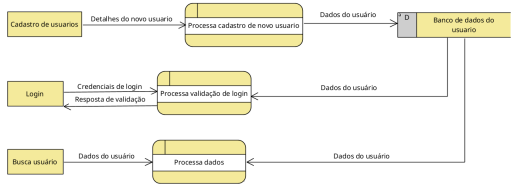
\includegraphics[width=12cm]{Pictures/diagram/loginNv1.png}
            \caption{Fluxo de dados do sistema Cadastro} \label{loginNV1}
      \end{center}
\end{figure}

\subsection{Diagramas DFD Login - entidade interno - Login}
O diagrama de fluxo de dados de nível 2 mostrado é o subsistema de login que possui a entidade de usuário onde o endereço de email e a senha do usuário são fornecidos, então as informações são processadas pelo sistema e verificam se as credenciais são válidas.
\begin{figure}[H]
      \begin{center}
            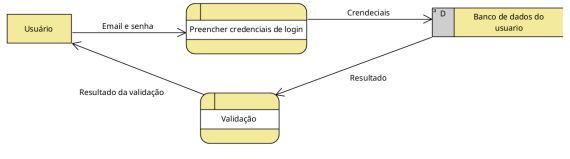
\includegraphics[width=12cm]{Pictures/diagram/loginNv2.png}
            \caption{Fluxo de dados do sistema Login} \label{loginNV2}
      \end{center}
\end{figure}
\section{Diagramas E-R}
O diagrama E-R é a representação gráfica de uma entidade relacional, onde a entidade é representada por um objeto e os relacionamentos são representados por relacionamentos. O diagrama E-R do sistema Buscalar completo é mostrado no exemplo dessa subseção.

O diagrama E-R do sistema de agenda possui as seguintes entidades: Usuário, agenda. Possui também os links: Usuários logado, onde o usuário pode cadastrar um ou mais agendas.


\section{Diagramas de Classes}
O diagrama de classes visa mostrar como o software está estruturado e como seus componentes estão interligados, ou seja, as operações que são realizadas entre eles.

\section{Diagramas Casos de uso}


Esta seção apresenta os casos de uso do sistema, cujo objetivo é mostrar as interações realizadas pelo usuário e as reações do sistema.


\subsection{Cadastro dos usuários}
\begin{enumerate}
      \item Preenchimento dos dados cadastrais do usuários;
      \item Login no sistema;
      \item Verificação de dados;
      \item Confirmação de dados;
      \item Gerar informações do usuário;
      \item Finalizar cadastro.
\end{enumerate}

\subsection{Criação de grupo}
\begin{enumerate}
      \item Cadastro de grupo no sistema;
      \item Preenchimento de dados;
      \item Informar valor do recurso para armazenamento;
      \item Atualizar dados do sistema;
      \item Finalizar cadastro de novos dados;
      \item Gerar relatório atual.
\end{enumerate}


\subsection{Excluir grupo}
\begin{enumerate}
      \item Atualizar dados do sistema;
      \item Deletar grupo para todos os usuários.

\end{enumerate}



\subsection{ Diagrama de Caso de Uso}
O diagrama a seguir pretende representar graficamente o caso de um "Serviço a um Usuário".
Cujo tem como objetivo representar o caso de uso do sistema e exibir informações sobre ele.

\begin{figure}[H]
      \begin{center}
            \caption{ Diagrama de caso de uso ao criar um grupo} \label{afp}
            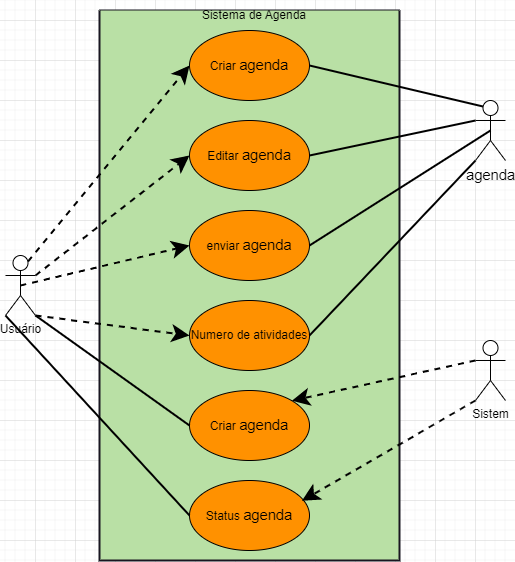
\includegraphics[width=15cm]{Pictures/diagram/casodeuso.drawio.png} \\


      \end{center}
\end{figure}

No subsistema de usuário, você pode alterar os detalhes do usuário, alterar senhas, adicionar fotos de perfil e editar informações pessoais, como nome, e-mail e telefone. E também é possível excluir a conta do usuário.
\begin{figure}[H]
      \begin{center}
            \caption{Diagrama de caso de uso de subsistema de usuário} \label{afp}
            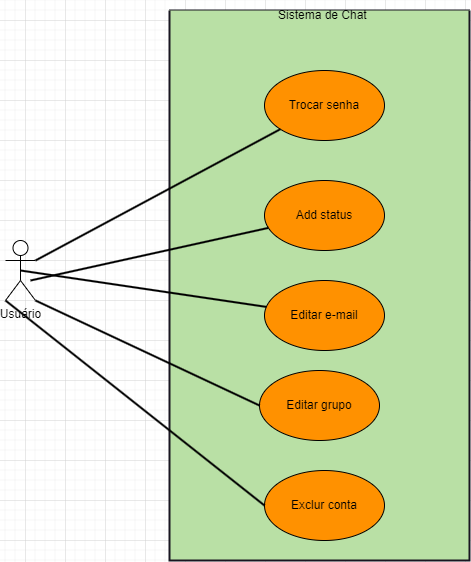
\includegraphics[width=15cm]{Pictures/diagram/casodeuso2.drawio.png} \\


      \end{center}
\end{figure}

\section{Diagramas Sequ\^{e}ncia}
O diagrama de sequência é uma solução de modelagem dinâmica popular em UML porque se concentra especificamente nas linhas de vida, ou nos processos e objetos que vivem ao mesmo tempo e nas mensagens trocadas entre eles para executar uma função antes que a linha de vida termine.

\begin{figure}[H]
      \begin{center}
            \caption{Diagrama de sequência de login} \label{afp}
            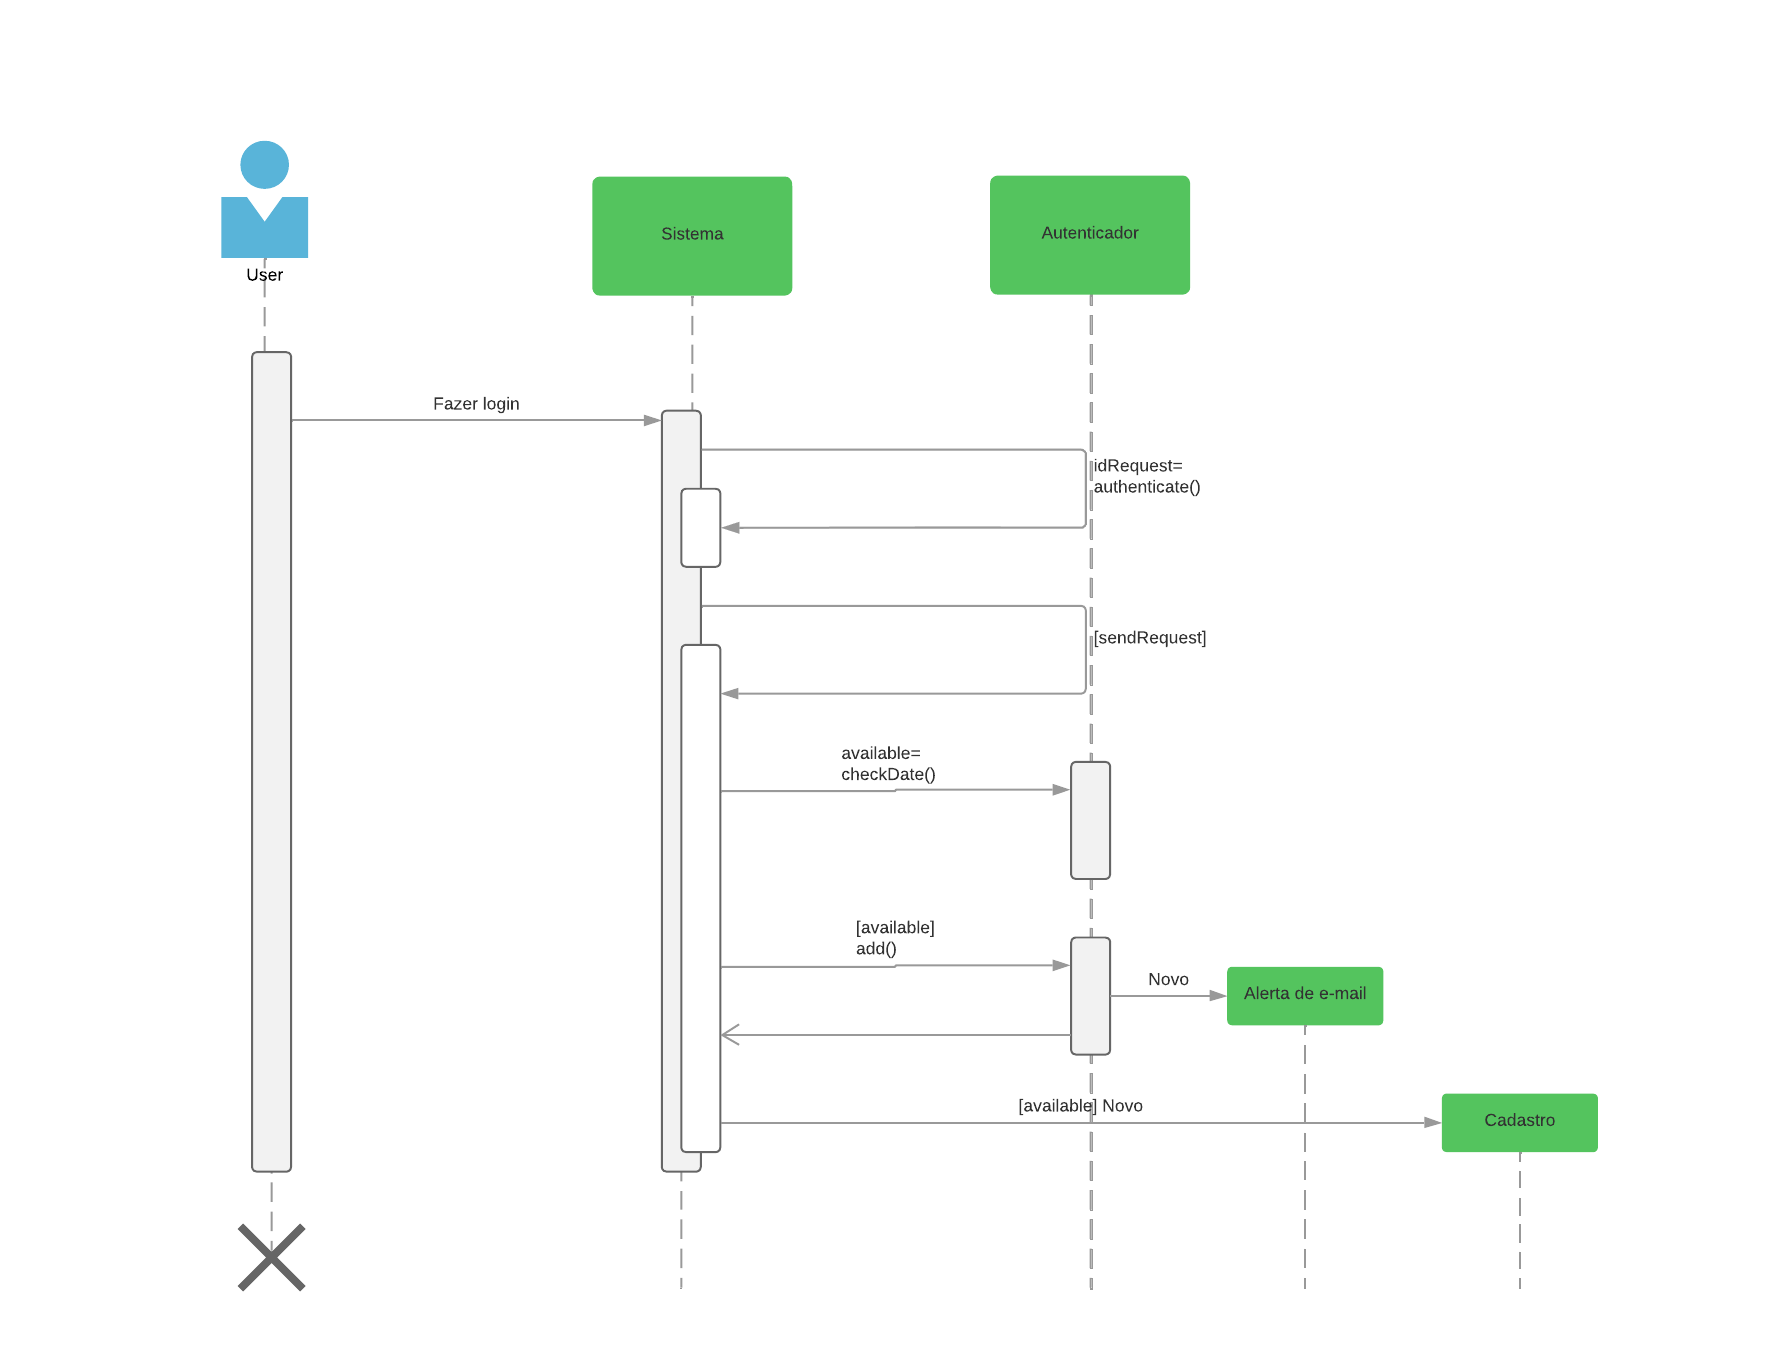
\includegraphics[width=15cm]{Pictures/diagram/sequencia.png} \\


      \end{center}
\end{figure}
Primeiro, o usuário faz login com o endereço de e-mail e a senha, depois o autenticador se comunica com o sistema e verifica se o usuário existe. Nesse caso, o sistema cria uma sessão para o usuário e retorna o acesso de verificação ou token (um código gerado pelo sistema e usado para realizar operações no sistema). Por fim, mostrará que o usuário está logado, então ele será redirecionado para a página principal.
\section{Diagramas de Atividades}
Um diagrama de atividades é essencialmente um fluxograma que mostra as atividades realizadas por um sistema. Assim, ilustra o fluxo ou sequência de ações executadas em um sistema.

\begin{figure}[H]
      \begin{center}
            \caption{Diagrama de atividade de login} \label{afp}
            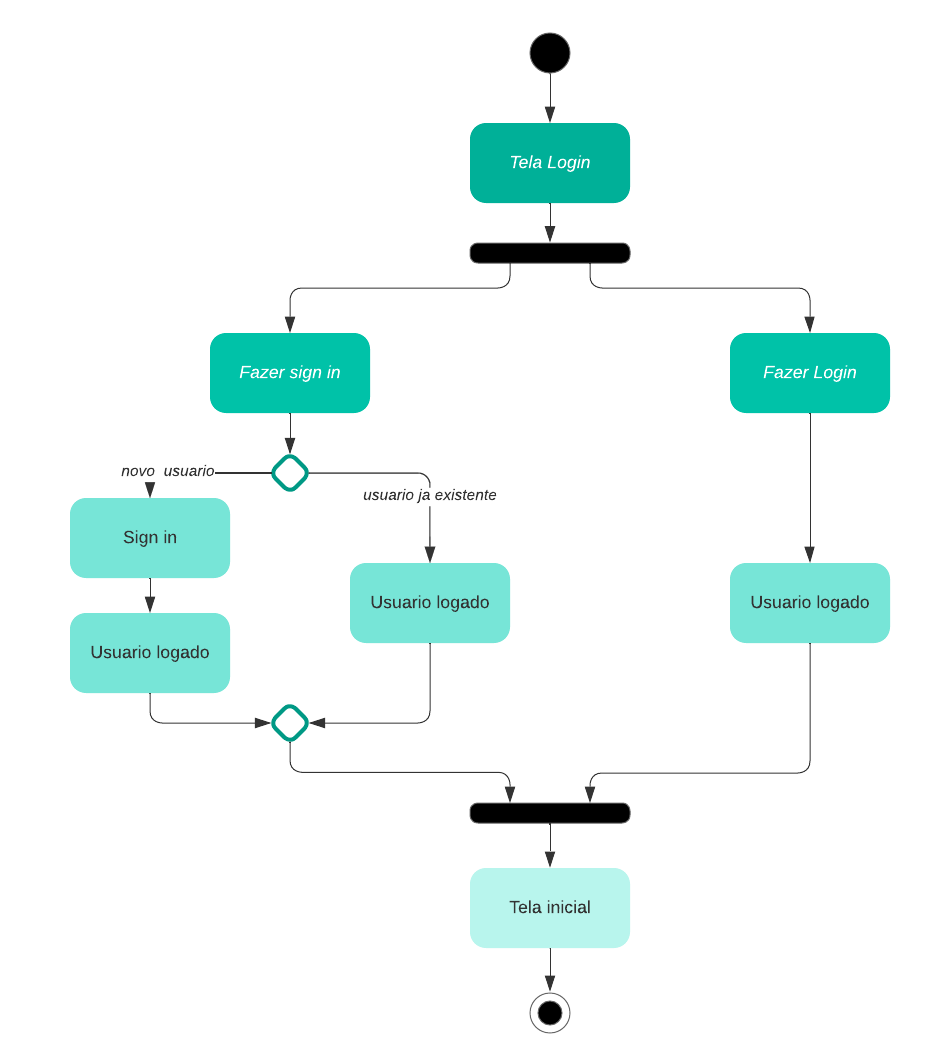
\includegraphics[width=15cm]{Pictures/diagram/atividade.png} \\


      \end{center}
\end{figure}
Primeiramente o usuário será levado para a tela de login onde será submetido a uma verificação se o usuário já está cadastrado, caso contrário o usuário será levado para a tela de cadastro do usuário, caso contrário será levado para a tela de login. Se o usuário estiver cadastrado, o usuário compartilhará o endereço de e-mail e a senha, então será realizada uma verificação, se o endereço de e-mail e a senha forem válidos, se não forem válidos, o usuário irá para a tela de login caso contrário será direcionado para a tela inicial do aplicativo.

Caso o usuário não esteja cadastrado, o usuário será direcionado para a tela de cadastro de usuário onde será enviado um formulário para o usuário preencher os dados onde será inserido o nome, e-mail e senha. As informações de e-mail e senha devem ser verificadas, caso o endereço de e-mail ou senha não seja válido, o usuário será direcionado para a tela de cadastro do usuário, caso contrário o cadastro será realizado e o usuário será direcionado para a tela de login.
\section{Diagramas Estado}
Um diagrama de estado, às vezes chamado de diagrama de máquina de estado, é um tipo de diagrama de comportamento na Unified Modeling Language (UML) que mostra transições entre diferentes objetos.
\begin{figure}[H]
      \begin{center}
            \caption{Diagrama de estado de login} \label{afp}
            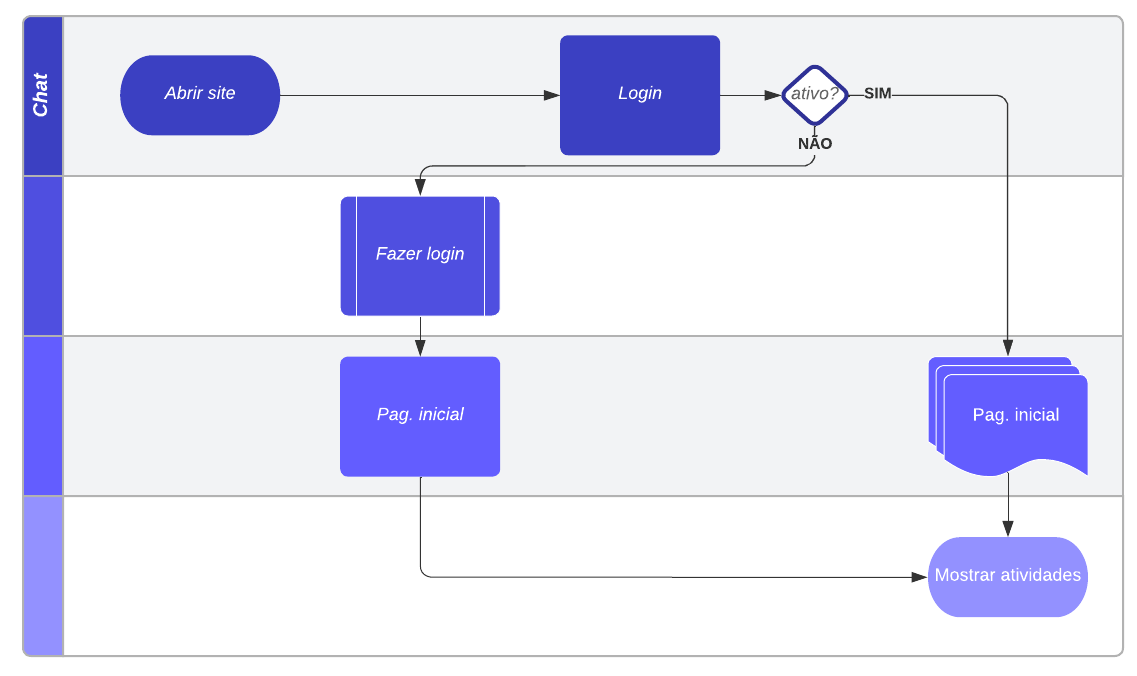
\includegraphics[width=15cm]{Pictures/diagram/estado.png} \\


      \end{center}
\end{figure}
Ao abrir o sistema ele verificará primeiro se o usuário está logado, se estiver o usuário será levado para a tela inicial, caso contrário para a tela de login onde será verificado se o usuário já está cadastrado, caso contrário o usuário será levado para a tela de cadastro do usuário, caso contrário, ele será direcionado para a tela de login. Se o usuário estiver cadastrado, o usuário fornecerá o e-mail e a senha, então será feita uma verificação, se o e-mail e a senha forem válidos, caso não sejam válidos, o usuário será levado para a tela de login. Caso o usuário não esteja cadastrado, o usuário será direcionado para a tela de cadastro de usuário onde será enviado um formulário para que o usuário preencha os dados onde estão inseridos nome, e-mail, telefone e senha.

As informações de e-mail, telefone e senha devem ser verificadas. Caso o endereço de e-mail, telefone ou senha não sejam válidos, o usuário será direcionado para a tela de cadastro do usuário, caso contrário o cadastro será realizado e o usuário será direcionado para a tela de login.
